\documentclass{article}
\usepackage{amsfonts}
\usepackage{amsmath}
\usepackage{mathtools}
\usepackage{systeme}
\usepackage{polynom}
\usepackage{pgfplots}
\everymath{\displaystyle}
\DeclarePairedDelimiter\ceil{\lceil}{\rceil}
\begin{document}
\begin{center}
\Large\textbf{Kodut\"o\"o nr. 5}\\
8. variant\\
\small{Joosep N\"aks}
\end{center}
\textbf{1.} Uurige j\"argmiste ridade koonduvust.
\begin{equation*}
\begin{aligned}
&\mathbf{a)} \sum_{k=1}^\infty\frac{((-1)^k+1)k}{k^2-k+1};\\
&\mathbf{b)} \sum_{k=0}^\infty\left(\frac{k^2+1}{(k+1)^2}\right)^{k^2}.\\
\end{aligned}
\end{equation*}
\textbf{Lahendus:}\\
a) Vaatlen k\~oigepealt jada $u_k=\frac{k}{k^2-k+1}$ summat 2st $\infty$ni, kuna $u_1$ on reaalarv, siis summa $u_k$ koondub 2st $\infty$ni parajasti siis, kui to koondub 1st $\infty$ni. Leian selle koonduvuse integraaltunnusega:
\begin{equation*}
\begin{aligned}
\int_2^\infty\frac{k}{k^2-k+1}=\frac{1}{2}\int_2^\infty\frac{2k}{k^2-k+1}dk
\end{aligned}
\end{equation*}
On teada, et integraal $\int_1^\infty\frac{1}{k^2}dk=1$ seega
\begin{equation*}
\begin{aligned}
\int_2^\infty\frac{1}{(k-1)^2}dk=1\\
\int_2^\infty\frac{1}{k^2-2k+1}dk=1
\end{aligned}
\end{equation*}
Kuna $k$ on alati positiivne, siis kui muuta nimetaja $k^2-2k+1$ nimetajaks $k^2-k+1$, muutub see suuremaks ehk integreeritav funktsioon muutub v\"aiksemaks ehk kui see on alati positiivne, on see integraal ikka koonduv. Et kontrollida, kas see on positiivne, leian selle nullkohad: $k_0=\frac{1\pm\sqrt{1-4}}{2}=\frac{1\pm\sqrt{-3}}{2}$ ehk nullkohti ei leidu. Vaatlen selle v\"a\"artust sisendil $k=0: 0^2-0+1=1$ ehk kuna nimetajal ei leidu nullkohti ega katkevuskohti ning ta on mingis punktis positiivne, on ta k\~oikjal positiivne. Seega on integraal $\int_2^\infty\frac{1}{k^2-k+1}dk$ koonduv ning ma saan ta juurde liita algsele vaadeldavale funktsioonile ilma selle koonduvust muutmata:
\begin{equation*}
\begin{aligned}
\frac{1}{2}\int_2^\infty\frac{2k}{k^2-k+1}+\frac{1}{k^2-k+1}dk=\frac{1}{2}\int_2^\infty\frac{2k+1}{k^2-k+1}dk
\end{aligned}
\end{equation*}
Kuna murru lugeja on nimetaja tuletis, on funktsiooni m\"a\"aramata integraal nimetaja naturaallogaritm:
\begin{equation*}
\begin{aligned}
\frac{1}{2}\int_2^\infty\frac{2k+1}{k^2-k+1}dk=\ln(k^2-k+1)\Big|_2^\infty=\lim_{c\to\infty}\ln(c^2-2+1)-\ln(2^2-2+1)=\infty
\end{aligned}
\end{equation*}
Seega kuna integraal ei koondu, ei koondu ka arvrida $\sum_{k=1}^\infty\frac{k}{k^2-k+1}$.\\
Vaatlen n\"u\"ud $\sum_{k=1}^\infty\frac{(-1)^kk}{k^2-k+1}=\sum_{k=1}^\infty(-1)^ku_k$ koonduvust Leibnizi tunnuse p\~ohjal. Selleks peab kehtima $\lim_{k\to\infty}\frac{k}{k^2-k+1}=0$, mis ka kehtib, ning jada $(u_k)$ peab olema kahanev. Selleks vaatlen suvalise liikme ja talle j\"argneva liikme vahet:
\begin{equation*}
\begin{aligned}
\frac{k+1}{(k+1)^2-(k+1)+1}-\frac{k}{k^2-k+1}&=\frac{k+1}{k^2+k+1}-\frac{k}{k^2-k+1}\\
&=\frac{k^3-k^2+k+k^2-k+1-k^3-k^2-k}{(k^2+k+1)(k^2-k+1)}\\
&=\frac{1-k^2-k}{(k^2+k+1)(k^2-k+1)}\\
\end{aligned}
\end{equation*}
Lugeja on $k\geq1$ korral negatiivne ning nimetajas $k^2+k+1$ on positiivsete $k$ korral alati positiivne ning $k^2-k+1$ kohta n\"aitasin lahenduse esimeses pooles, et see on alati positiivne, seega on saadud murd k\~oigi $k\in\mathbb{N}$ korral negatiivne ehk $(u_k)$ on kahanev. Seega on Leibnizi eeldused t\"aidetud ning $\sum_{k=1}^\infty\frac{(-1)^kk}{k^2-k+1}$ koondub.\\
Kokkuv\~ottes $\sum_{k=1}^\infty\frac{((-1)^k+1)k}{k^2-k+1}$ hajub kuna see on hajuva rea ja koonduva rea summa.
\pagebreak\\
b) Kasutan Cauchy koonduvustunnust. Olgu $\displaystyle u_k=\left(\frac{k^2+1}{(k+1)^2}\right)^{k^2}$. Selleks, et $u_k$ summa koonduks, peab leiduma $c:=\lim_{k\to\infty}\sqrt[k]{|u_k|}$ ning peab kehtima $c<1$.
\begin{equation*}
\begin{aligned}
c&=\lim_{k\to\infty}\sqrt[k]{\left(\frac{k^2+1}{(k+1)^2}\right)^{k^2}}\\
&=\lim_{k\to\infty}\left(\frac{k^2+1}{(k+1)^2}\right)^{k}\\
&=\lim_{k\to\infty}\left(\frac{k^2+1+2k-2k}{k^2+2k+1}\right)^{k}\\
&=\lim_{k\to\infty}\left(1-\frac{2k}{(k+1)^2}\right)^{k}\\
&\text{Teen muutujavahetuse }u=k+1:\\
&=\lim_{k\to\infty}\left(1-\frac{2(u-1)}{u^2}\right)^{u-1}\\
&=\lim_{k\to\infty}\left(1-\frac{2}{u}+\frac{2}{u^2}\right)^{u-1}\\
&\text{Teen muutujavahetuse }v=-\frac{u}{2}:\\
&=\lim_{k\to\infty}\left(1+\frac{1}{v}+\frac{1}{2v^2}\right)^{-2v-1}\\
&=e^{-2}
\end{aligned}
\end{equation*}
Kuna see piirv\"a\"artus leidub, on Cauchy koonduvustunnuse p\~ohjal $u_k$ koonduv.
\pagebreak\\
\textbf{2.} Leidke m\"a\"aramata integraal astmereana ja arvutage see j\"arel m\"a\"aratud integraal
\begin{equation*}
\int_0^1\cos x^2dx \text{ t\"apsusega }10^{-4}.
\end{equation*}
\textbf{Lahendus:}\\
Loon Taylori rea punkti $a=0$ \"umber. Taylori rea \"uldliiget saab esitada kujul $P_n(x)=\frac{(\cos a)^{(n)}x}{n!}$. M\"arkan, et paarituarvuliste $n$ korral on $(\cos a)^{(n)}=\pm\sin 0=0$. Seega saab neid liikmeid ignoreerida. paarisarvuliste $n$ korral on $(\cos a)^{(n)}$ vaheldumisi $\pm1$. Seega saab \"uldliikme \"umber kirjutada kui
\begin{equation*}
P_n(x)=\left\{
\begin{aligned}
&\frac{(-1)^{\frac{n}{2}}x}{n!}, && kui\ n=2k,\ k\in\mathbb{N}\\
&0, && kui\ n=2k+1,\ k\in\mathbb{N}
\end{aligned}
\right.
\end{equation*}
Seega kui iga teine $n$ vahele j\"atta, saame summa $\cos(x)=\sum_{n=0}^\infty(-1)^n\frac{x^{2n}}{(2n)!}$ ehk integreeritavat funktsiooni saab esitada kui $\cos(x^2)=\sum_{n=0}^\infty(-1)^n\frac{x^{4n}}{(2n)!}$. Kontrollin funktsionaaljada $f_n(x)=(-1)^n\frac{x^{4n}}{(2n)!}$ \"uhtlast koonduvust hulgas $[0,1]$. Selleks kasutan Weierstrassi koonduvustunnust, loon arvrea $u_k = (-1)^n\frac{1}{(2n)!}$, mis on iga $x$ ja $n$ korral suurem v\~oi v\~ordne $f_n(x)$ga, kuna $f_n(x)$ s\~oltub $x$st v\~ordeliselt. Leibnizi tunnnuse p\~ohjal $\sum_{n=0}^\infty u_n$ koondub, kuna $\frac{1}{(2n)!}$ piirv\"a\"atrus l\"aheneb l\~opmatuse juures 0le. Kuna $\sum_{n=0}^\infty u_n$ koondub siis Weierstrassi koonduvustunnuse p\~ohjal funktsionaaljada $f_n(x)$ koondub \"uhtlaselt.\\
Kuna $f_n(x)$ koondub \"uhtlaselt, saan loengukonspekti teoreemi 6.34 p\~ohjal vahetada integraali ja summa funktsionaaljada ees \"ara:
\begin{equation*}
\int_0^1\sum_{n=0}^\infty(-1)^n\frac{x^{4n}}{(2n)!}dx=\sum_{n=0}^\infty \int_0^1(-1)^n\frac{x^{4n}}{(2n)!}dx=\sum_{n=0}^\infty (-1)^n\frac{x^{4n+1}}{(4n+1)(2n)!}\Big|_0^1=\sum_{n=0}^\infty (-1)^n\frac{1}{(4n+1)(2n)!}
\end{equation*}
Kuna tegu on Taylori reaga, esitub summa j\"a\"akllige kujul $R_n(x^2)=\frac{(\cos c^2)^{(n+1)}}{(n+1)!}x^{2(n+1)},$ $\ c\in[0,1]$. Kuna selle funktsiooni p\"o\"ordfunktsiooni on raske leida, proovin $n$ v\"a\"artuseid l\"abi. Kuna paarituarvuliste $n$ korral on rea liikmed 0d, saab $n$ v\"a\"artuseid \"ule \"uhe proovida kasutan paarituarvulisi $n$ v\"a\"artuseid et lihtsustada arvutamist. Kuna j\"a\"akliige s\~oltub v\~ordeliselt $x$st, kasutan $x=1$. Kuna koosinuse paarisarvulised tuletised on koosinused ning koosinuse suurim v\"a\"artus on 1, kasutan seda hindamiseks. Eesm\"ark on saavutada t\"apsus $10^{-4}$ ehk et j\"a\"akliige v\"aiksem kui $\frac{1}{10000}$
\begin{equation*}
\begin{aligned}
R_1(x)&=\frac{1}{2!}1^{2}=\frac{1}{2}>\frac{1}{10000}\\
R_3(x)&=\frac{1}{4!}1^4=\frac{1}{24}>\frac{1}{10000}\\
R_5(x)&=\frac{1}{6!}1^6=\frac{1}{720}>\frac{1}{10000}\\
R_7(x)&=\frac{1}{8!}1^8=\frac{1}{40320}<\frac{1}{10000}\\
\end{aligned}
\end{equation*}
Seega on sobiva t\"apsusega summa 
\begin{equation*}
\begin{aligned}
S&=(-1)^0\frac{1}{(4\cdot0+1)(2*0)!}+(-1)^1\frac{1}{(4\cdot1+1)(2\cdot1)!}+(-1)^2\frac{1}{(4\cdot2+1)(2\cdot2)!}+(-1)^3\frac{1}{(4\cdot3+1)(2\cdot3)!}\\
&=1-\frac{1}{10}+\frac{1}{216}-\frac{1}{9360}\\
&=\frac{25399}{28080}\approx0.9045
\end{aligned}
\end{equation*}
\pagebreak\\
\textbf{3.} Uurige rea
\begin{equation*}
\sum_{k=0}^\infty\frac{kx}{1+k^5x^2}
\end{equation*}
\"uhtlast koonduvust piirkonnas $(-\infty,\infty)$.\\
Koostage arvuti abil joonis, kus on \"uhes teljestikus n\"aha rea osasummade $S_3(x), S_5(x)$ ja $S_{100}(x)$ graafikud piirkonnas $x\in[-0.2,0.2]$.\\
\textbf{Lahendus:}
Kasutan Weierstrassi koonduvustunnust. See \"utleb, et kui leidub selline arvrida $u_k$, et $|f_k(x)|\leq u_k$ iga $x\in\mathbb{R}$ ja iga $k\in\mathbb{N}$ korral ning $\sum_{k=1}^\infty u_k<\infty$, siis funktsionaalrida $\sum_{k=1}^\infty f_k$ koondub hulgas $\mathbb{R}$ \"uhtlaselt ja absoluutselt. Sobiva arvrea leidmiseks leian $f_k(x)=\frac{kx}{1+k^5x^2}$ maksimaalse v\"a\"artuse iga $k\in\mathbb{N}$ juures. Selleks v\~otan $f_k(x)$ tuletise $x$ j\"argi:
\begin{equation*}
\frac{\partial}{\partial x}\left(\frac{kx}{1+k^5x^2}\right)=\frac{k(1-k^5x^2)-2k^5x\cdot kx}{(1+k^5x^2)^2}=\frac{k(1-k^5x^2)}{(1+k^5x^2)^2}
\end{equation*}
Selleks, et tuletis 0 oleks, peab tema lugeja olema null.
\begin{equation*}
\begin{aligned}
k(1-k^5x_0^2)=0\\
1=k^5x_0^2\\
x_0=\pm k^{-\frac{5}{2}}
\end{aligned}
\end{equation*}
Funktsiooni $f_k(x)$ ainus katkevuskoht saaks olla siis, kui nimetaja oleks null ehk $1+k^5x^2=0$, kuid $k$ on alati positiivne ja $x^2$ on alati positiivne seega nimetaja ei saa 0 olla. Seega on $f_k(x)$ globaalne maksimum l\~opmatuses, miinus l\~opmatuses, $k^{\frac{5}{2}}$ juures v\~oi $-k^{\frac{5}{2}}$ juures. Proovin need l\"abi:
\begin{equation*}
\begin{aligned}
\lim_{x\to\infty}\frac{kx}{1+k^5x^2}&=\lim_{x\to\infty}\frac{k}{2k^5x}=0\\
\lim_{x\to-\infty}\frac{kx}{1+k^5x^2}&=\lim_{x\to-\infty}\frac{k}{2k^5x}=0\\
x=k^{-\frac{5}{2}}&: \frac{kk^{-\frac{5}{2}}}{1+k^5(k^{-\frac{5}{2}})^2}=\frac{k^{-\frac{3}{2}}}{2}\\
x=-k^{-\frac{5}{2}}&: \frac{k(-k^{-\frac{5}{2}})}{1+k^5(-k^{-\frac{5}{2}})^2}=-\frac{k^{-\frac{3}{2}}}{2}
\end{aligned}
\end{equation*}
Seega on $|f_k(x)|$ maksimaalne v\"a\"artus $f_k(x_{max})=\frac{k^{-\frac{3}{2}}}{2}:=u_k$.\\
Kuna $u_k$ on kahanev ja mitte negatiivne, leian integraaltunnusega, kas $u_k$ koondub:
\begin{equation*}
\begin{aligned}
\int_1^\infty\frac{k^{-\frac{3}{2}}}{2}dk=\frac{k^{-\frac{1}{2}}}{2}\Big|_1^\infty=\lim_{c\to\infty}\frac{c^{-\frac{1}{2}}-1^{-\frac{1}{2}}}{2}=\frac{1}{2}
\end{aligned}
\end{equation*}
Seega kuna $u_k$ summa koondub, koondub ka $f_k(x)$ \"uhtlaselt.
Joonis osasummadega:\\
\begin{center}
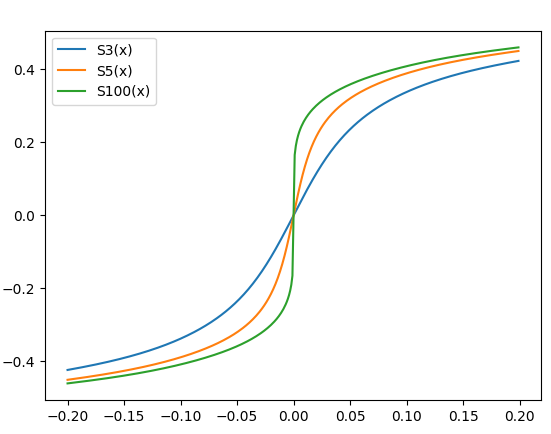
\includegraphics[scale=0.5]{graaf.png}
\end{center}
\end{document}